\documentclass[tikz,border=8pt]{standalone}
\usetikzlibrary{arrows.meta}
\begin{document}
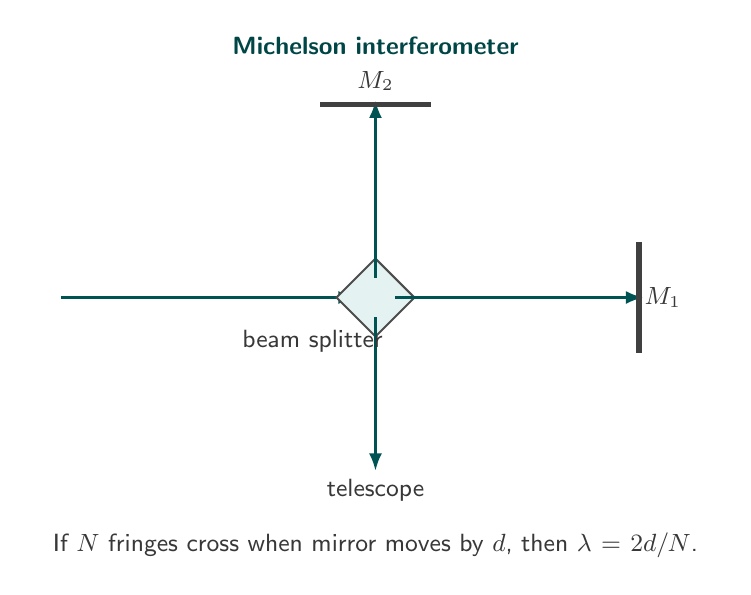
\begin{tikzpicture}[
  ray/.style={-{Latex[length=2.2mm]},draw=teal!65!black,line width=0.9pt},
  line/.style={draw=black!70,line width=0.75pt},
  mirror/.style={draw=black!75,line width=2pt},
  label/.style={font=\sffamily\small,text=black!78},
  title/.style={font=\sffamily\bfseries\small,text=teal!55!black},
]
\node[title] at (0,3.2) {Michelson interferometer};
\draw[ray] (-4,0)--(-0.25,0);
\draw[line,fill=teal!10,rotate=45] (-0.35,-0.35) rectangle (0.35,0.35);
\draw[ray] (0.25,0)--(3.4,0);
\draw[ray] (0,0.25)--(0,2.5);
\draw[ray] (0,-0.25)--(0,-2.2);
\draw[mirror] (3.35,-0.7)--(3.35,0.7);
\draw[mirror] (-0.7,2.45)--(0.7,2.45);
\node[label] at (3.65,0) {$M_1$};
\node[label] at (0,2.75) {$M_2$};
\node[label] at (-0.8,-0.55) {beam splitter};
\node[label] at (0,-2.45) {telescope};
\node[label,align=center,text width=8.6cm] at (0,-3.15)
  {If $N$ fringes cross when mirror moves by $d$, then $\lambda=2d/N$.};
\end{tikzpicture}
\end{document}
